\documentclass{article}
\usepackage{graphicx}
\usepackage[czech]{babel}
\usepackage{project}
\usepackage{float}
\addto\captionsenglish{\renewcommand{\figurename}{Fig.}}
\renewcommand*{\lstlistlistingname}{List of Programs}
\graphicspath{ {./images/} }
\def\projectauthor{Matyáš Peroutík\\256371}
\def\projecttitle{Závěrečný projekt}
\def\projectprogramme{Kurz \\ BPC-UKB}
\def\projectmonth{\today}
% SECTION STYLE
\setcounter{tocdepth}{2}                            
\setcounter{secnumdepth}{3}


\makeatletter
\renewcommand{\@seccntformat}[1]{}
\makeatother
 	
\begin{document}
    \prefrontmatter
    \newpage
    \pagenumbering{arabic} 
    \tableofcontents
    \begingroup
        \let\clearpage\relax
        \vspace*{20pt}
        \listoftables
        \vspace*{20pt}
        \listoffigures
        \vspace*{20pt}
    \endgroup
    \addtolength{\parskip}{\baselineskip}
    \renewcommand{\sectionmark}[1]{\markright{\ #1}}
   	\newpage

	\section{Úkol 1}
	   	\paragraph{} 
	   	V této části zadání jsem měl ověřit, zda je systém, na který budeme sestrojovat regulátor lineární, a zároven časově invarientní (LTI). Pro to, aby byl systém lineární, musí být splněny podmínky homogenity a aditivy.
	   	\subsection{Ověření homogenity}
	   	\paragraph{}
	   		Homogenitu ověříme tak, že původní signál vynásobíme libovolnou konstantou (v našem případě zvolíme k=0.5) a pokud je systém homogenní, tak všechny jeho hodnoty v čase t budou k-krát větší. Toto ověříme pomocí kurzorů v grafu funkce systému a funkce systému krát konstanta pomocí kurzorů.
	   		\begin{figure}[H]
	   		 \begin{minipage}[b]{.45\textwidth}
    \centering
    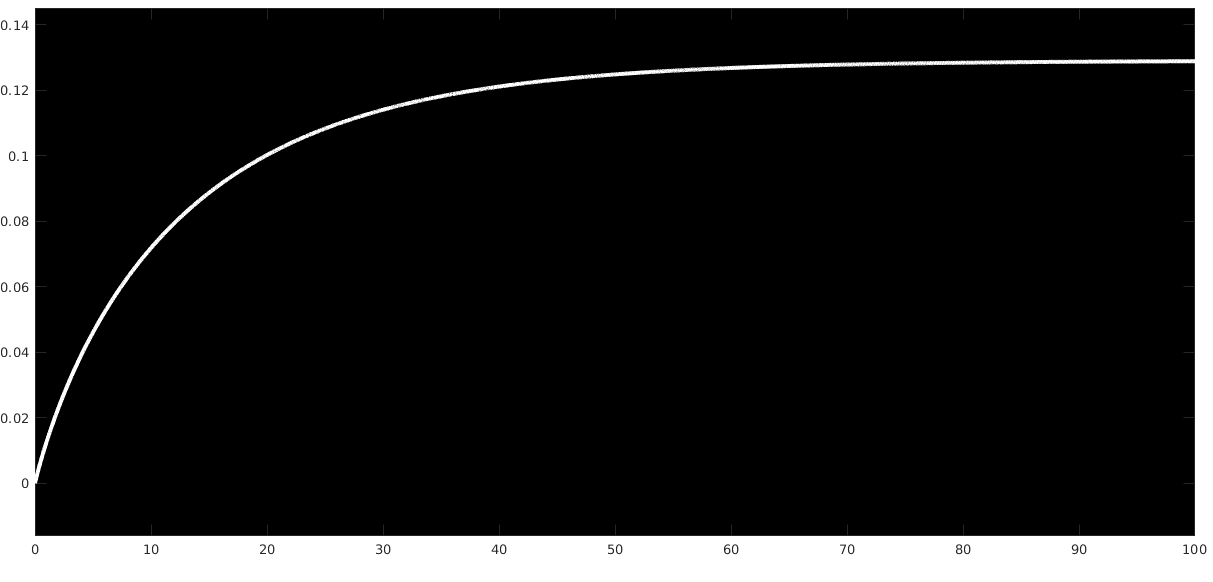
\includegraphics[width=\linewidth]{ukol1k1}
    \caption{Závislost výšky hladiny regulovaného systému v závislosti na čase s průtokem vynásobeným konst. k = 1}
  \end{minipage}\hfill
  \begin{minipage}[b]{.45\textwidth}
    \centering
    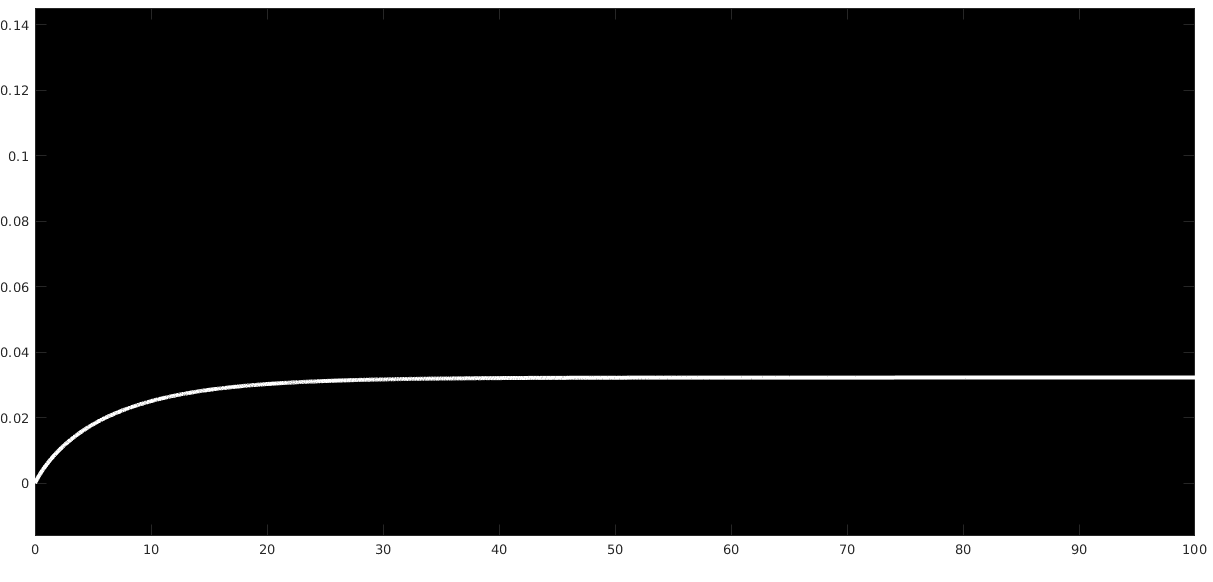
\includegraphics[width=\linewidth]{ukol1k05}
    \caption{Závislost výšky hladiny regulovaného systému v závislosti na čase s průtokem vynásobeným konst. k = 0.5}
  \end{minipage}
	   		\end{figure}
	   		
	   		\indent Na těchto grafek se stejným měřítkem můžeme vidět, že pokud vstupní signál (průtok) změníme k-krát, tak výsledná hodnota se k-krát nezmění. Tudíž systém homogenní není.
	   		
	   			   		
	  	\subsection{Ověření aditivy}
	  	\paragraph{}
	  		Aditiva znamená, že pokud budeme mít dva různé vstupní signály u1 a u2, a dva různé výstupní signály y1 a y2, tak výstupní signál y12 pro vstuoní sígnál u12 = u1 + u2 bude roven součtu výstupních signálů odpovídajícím sečteným vstupním signálům, resp. y12 = y1 + y2. Toto si ověříme tím, že si vygrafujeme signály y1, y2 ,y12, a rozdíl těchto signálů (y12-y1-y2). Pokud bude rozdíl pořád roven 0, systém můžeme uvažovat za aditivní. Pro ověření jsem zvolil, že průběhy y1 a y2 budou oba začínat v časovém okamžiku 0. y1 (bílá barva)bude mít velikost 0.0005, y2 (modrá barva) bude mít velikost 0.001, a tím pádem velikost průběhu y12 (zelená barva) bude 0.0015.
	  		
	  		\begin{figure}[H]
	  		\centering
	  		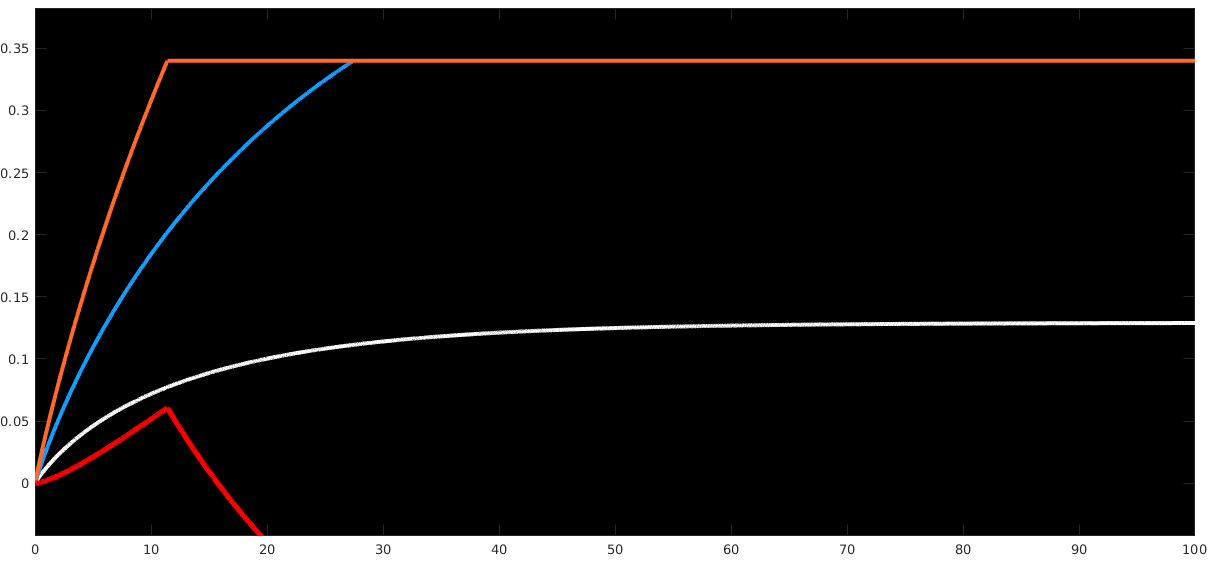
\includegraphics[width=\textwidth]{ukol1aditiv}
	  		\caption{Graf vyvracející adivitu}
	  		\end{figure}
	   		
	   	\paragraph{}
	   	Z tohoto grafu lze vidět, že rozdíl hodnot (červená barva) není roven nule, a tím pádem systém není aditivní.
	   	
	   	\subsection{OVěření časové invarientnosti}
	   	Časově invarientí systém je takový, u kterého nezávisí na tom, v jakém časovém okamžiku na něj začneme působit vstupní veličinou. Toto lze ověřít tak, že budeme mít dva shodné signály y1 a y2, a signál y2 zpozdíme např. o 10s. Toto je zobrazené na následujícím grafu.
	  		\begin{figure}[H]
	  		\centering
	  		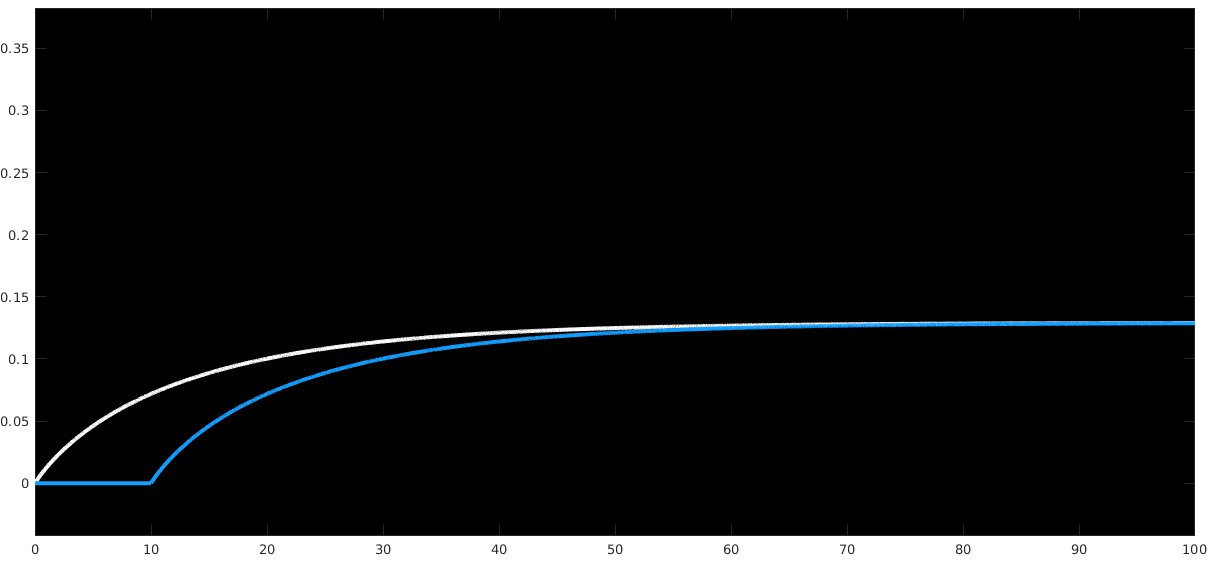
\includegraphics[width=\textwidth]{ukol1invar}
	  		\caption{Graf dokazující časovou invarientnost obvodu}
	  		\end{figure}
   	\paragraph{}
   	Na tomto grafu můžeme vidět, že pokud zpozdíme vstupní signál o 10s, tak nám to jeho tvar či velikost ustálené hodnoty nezmění. Systém je tedy časově invarientní.
   	
   	\subsection{Vyhodnocení}
   	\paragraph{}
   	Z těchto zjištěných výsledků můžeme tvrdit, že se nejedná o LTI systém, protože ačkoliv je systém časově invarientní, tak systém není lineární, ale je nelineární, protože není splněna ani podmínka aditivy systému, ani homogenity.
   	
   	\section{Úkol 2}
	\paragraph{}
		V tomto úkolu zjišťujeme parametry předchozího systému, při čemž tvrdíme, že předchozí systém je LTI při konstantním vstupu 0.5l/s. Na základě zjištěných parametrů poté určím parametry náhradního lineárního modelu.
		
		\subsection{Zjištění parametrů LTI systému}
		\paragraph{}
		V tomto úkolu je požadováno zobrazit přechodovou charakteristiku obou systémů.
		
   	
   		\begin{figure}[H]
   			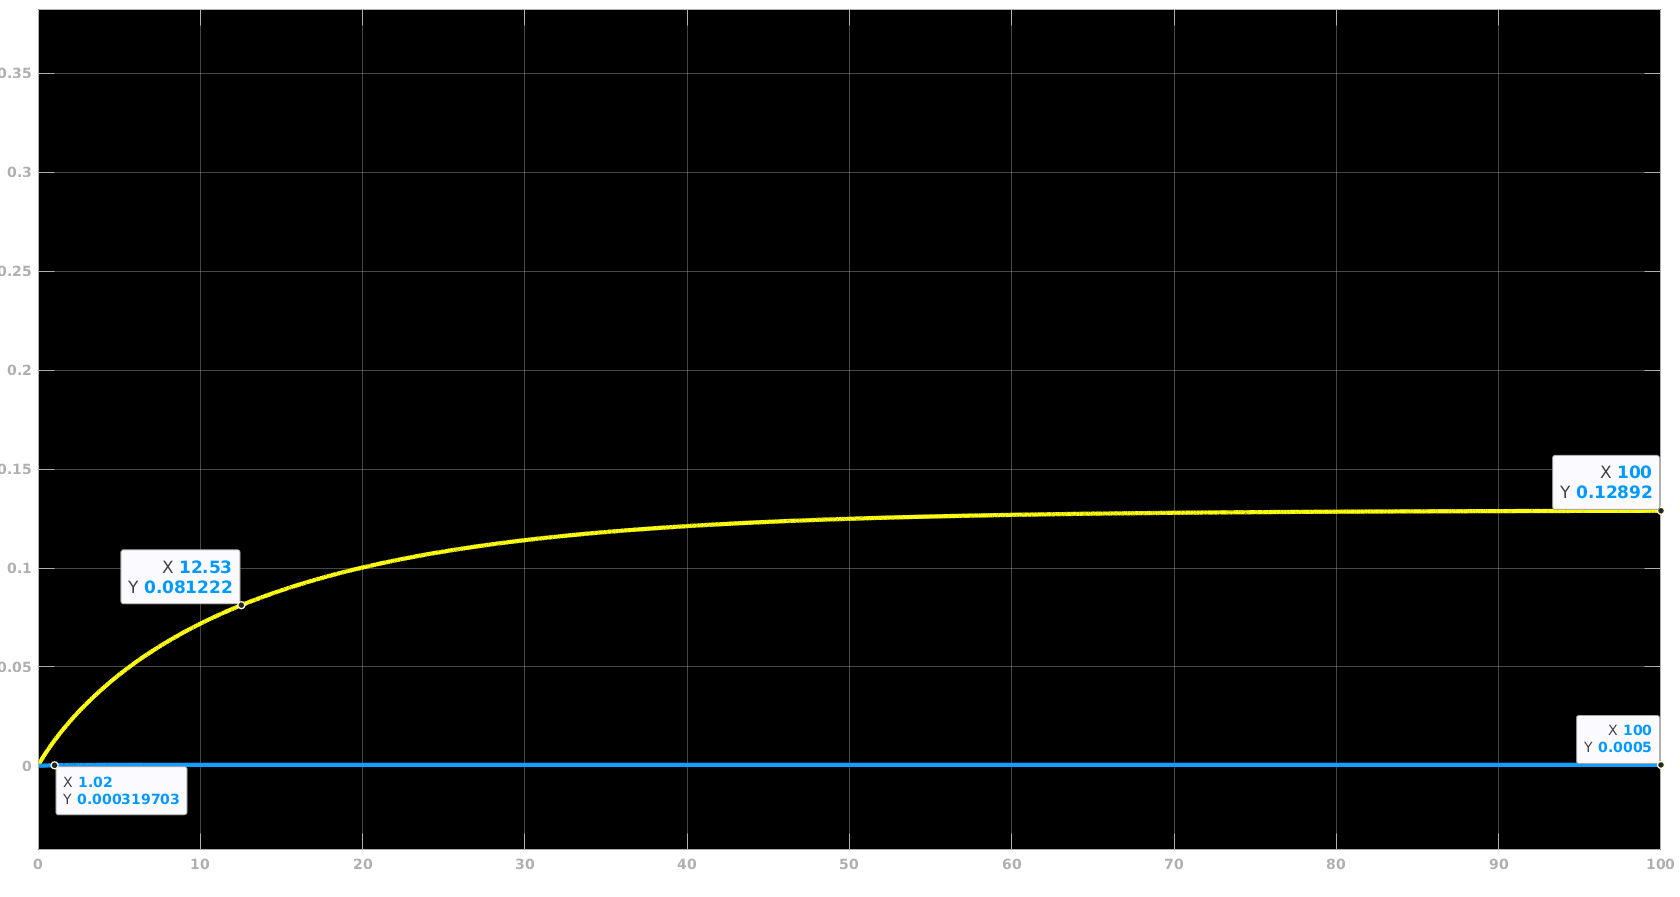
\includegraphics[width = \textwidth]{ukol2meas1}
   			\caption{Graf přechodové charakteristiky nelineární soustavy (žlutá) a jejího nenastaveného modelu (modrá) se zobrazenými hodnotami maxima a hodnotě za dobu $\tau$}
	   	\end{figure}
   	
		\paragraph{}
		   	Z tohoto grafu lze vidět, že systém má jeden akumulátor energie, a má i disipativní prvek, který způsobuje autoregulaci. Tudíž se jedná o systém 1. řádu se ztrátami. 
		   	\indent Pro zjištění parametru zesílení \textit{K} LTI (žlutého) průběhu je potřeba znát ustálenou hodnotu tohoto průběhu. To je zobrazeno v předešlém grafu. Zesílení K poté spočteme následovně:
		   	\begin{equation}
		   	\label{eqn:gain}
		   	K = \frac{y_{ust}}{u} = \frac{0.12892}{0.0005} = 257.84
		   	\end{equation}
   	\indent Pro zjištění časové konstanty $\tau$ jsem vypočetl jako 0.637$y_{ust}$. Toto je možné, protože se jedná o systém 1. řádu
   			\begin{equation}
   			\label{eqn:tau}
   			y(\tau) = 0.637 \cdot y_{ust} = 0.637 \cdot 0.12892 = 0.082122
   			\end{equation}
   			
   	\indent Tuto hodnotu výstupní veličiny jsem označil v grafu. Jelikož se do obvodu pustila vstupní veličina v časovém okamžiku nula, můžeme uvažovat časový okamžik ve chvíli, kdy dosáhne y vypočtené hodnoty. Potom je tedy časová konstanta $\tau$ = 12.53s.
 	\indent Pokud dosadíme tedy za hodnoty K a T u lineárního modelu této soustavy dostaneme následující graf:
 	
 	\begin{figure}[H]
 	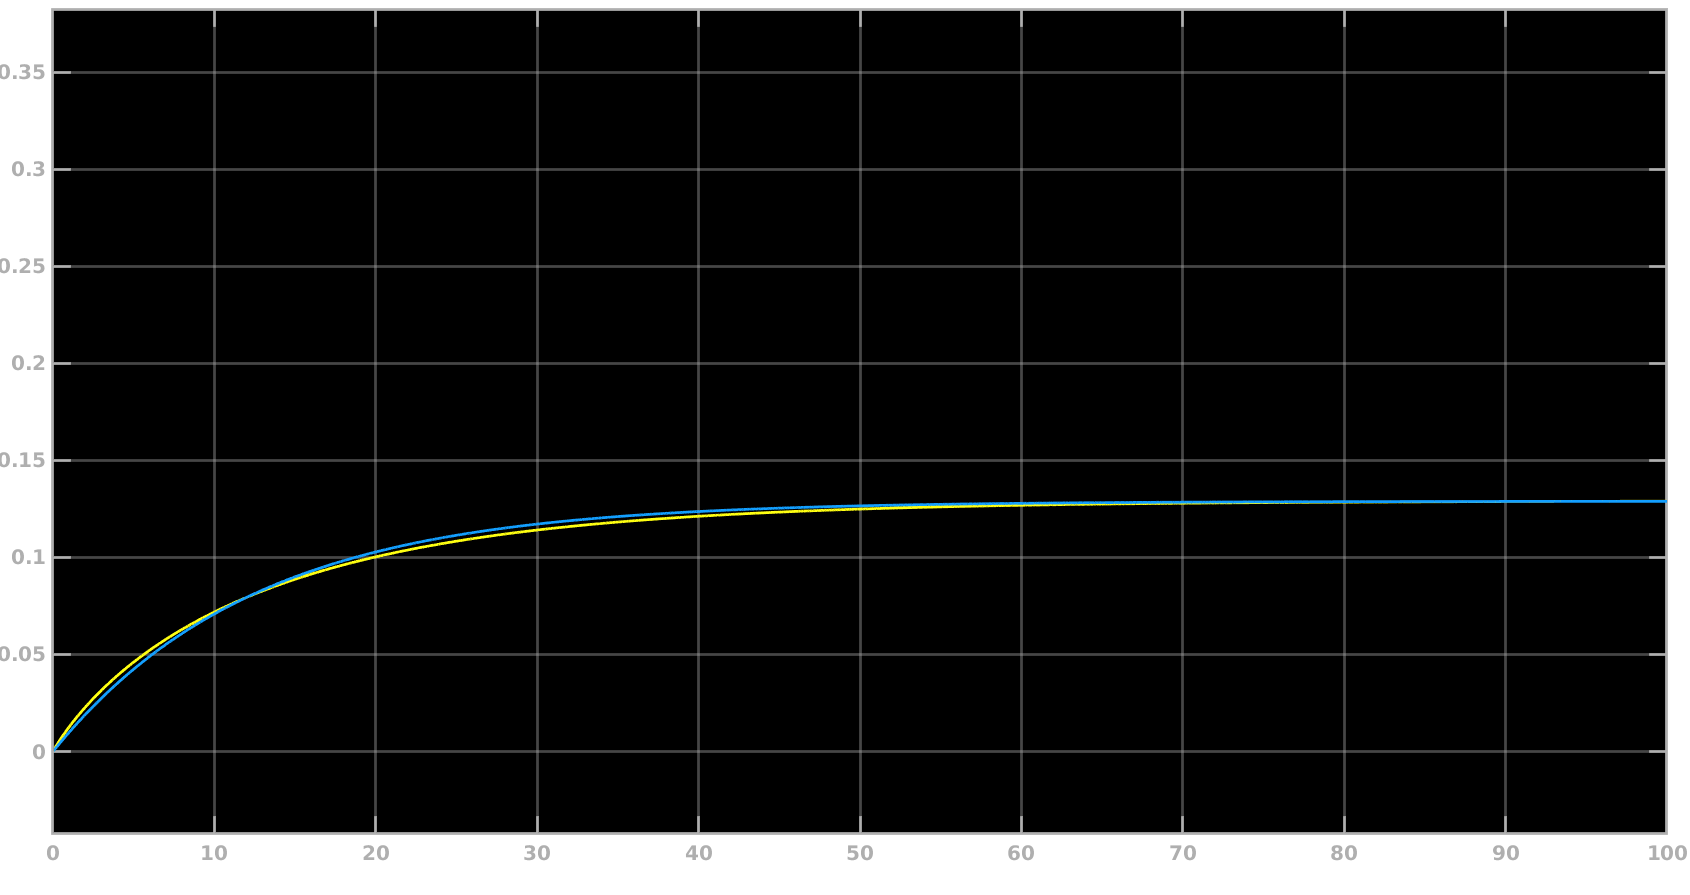
\includegraphics[width=\textwidth]{ukol2meas2}
 	\caption{Graf přechodové charakteristiky nelineární soustavy (žlutá) a jejího nastaveného lineárního modelu (modrá) pomocí zjištěných hodnot z výpočtů (\ref{eqn:tau}) a (\ref{eqn:gain})}
 	\end{figure}
   			
   	
   	\section{Úkol 3}
   	\paragraph{}
   		V tomto úkolu budeme regulovat model soustavy pomocí idealního PID regulátoru. Pro realizaci této regulace je nutné stanovit si, které veličiny jsou které, a jaký mají rozměr.
   		
   		% Please add the following required packages to your document preamble:
% \usepackage{graphicx}
\begin{table}[H]
\centering
\resizebox{0.7\textwidth}{!}{%
\begin{tabular}{|l|l|l|l|}
\hline
\textbf{Značka} & \textbf{Popis}               & \textbf{Veličina} & \textbf{Jednotka} \\ \hline
\textit{w(t)}   & Požadovaná hodnota výsky     & výška             & {[}m{]}           \\ \hline
\textit{e(t)}   & Odchylka od požadované výšky & výška             & {[}m{]}           \\ \hline
\textit{u(t)}   & Akční zásah - vstup          & průtok            & {[}m3/s{]}        \\ \hline
\textit{y(t)}   & Regulovaná veličina - výstup & výska             & {[}m{]}           \\ \hline
\end{tabular}%
}
\caption{Veličiny regulační smyčky}
\label{tab:regtable}
\end{table}
   	
\subsection{Regulace pomocí složky P}   	
   	
   	\indent Experimentálně jsem následně začal nastavovat jednotlivé složky regulátoru. Jako první jsem začal nastavovat pouze složku P. Tu jsem nastavil na hodnotu 0.005, protože je to nejvyšší hodnota, u kterého je maximální průtok, který uvažuji (resp. 0.0005m3/s).
   	
   	\begin{figure}[H]
	   		 \begin{minipage}[b]{.45\textwidth}
    \centering
    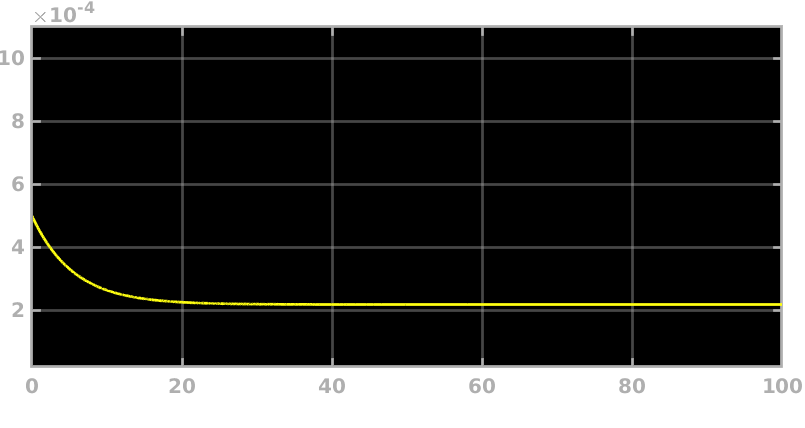
\includegraphics[width=\linewidth]{ukol3P0005u}
    \caption{Průběh akčního zásahu u(t) ovládaným pouze P regulátorem s hodnotou P = 0.005}
  \end{minipage}\hfill
  \begin{minipage}[b]{.45\textwidth}
    \centering
    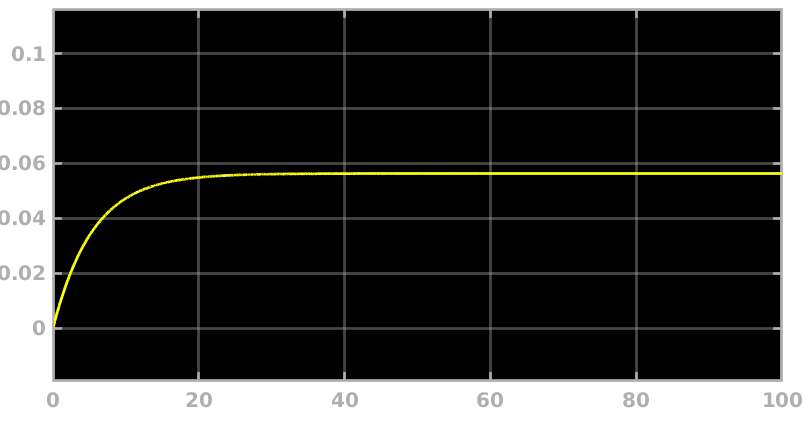
\includegraphics[width=\linewidth]{ukol3P0005y}
    \caption{Průběh výšky hladiny systému y(t) regulovaným pouze P regulátorem s hodnotou P = 0.005}
    \label{img:hladinaP0005}
  \end{minipage}
	   		\end{figure}
   	
	
	\indent Jak lze z Obrázku~\ref{img:hladinaP0005} sledovat, tak P regulátor \textbf{NENÍ} schopen naregulovat požadovanou veličinu. Pokud bychom nastavili složku P 1, průtok by byl nereálný (0.1m3/s). Pokud by byla hodnota P nižší, ustálená hodnota výsledné hladiny by se táké snížíla. Pomocí regulátoru P jsme schopni v tomto případě naregulovat výšku pouze na hodnotu 0.05632m z požadované výsky 0.1m. 
	

\subsection{Regulace pomocí složek PD}

	\indent Jelikož složka P reaguje na změnu požadované odchylky, tak se jeho průběh nebude moc lišit od regulace pomocí složky P. Nejvyšší změna nastave v čase, kdy zastavíme požadovanou hodnotu, a následně pouze urychlí, za jak dlouho výsledný průběh zakonverguje. Ponecháme-li konstantu P z minulé úlohy stejnou, můžeme experimentálně nastavit konstantu D.	
	
	
	\begin{figure}[H]
	   		 \begin{minipage}[b]{.45\textwidth}
    \centering
    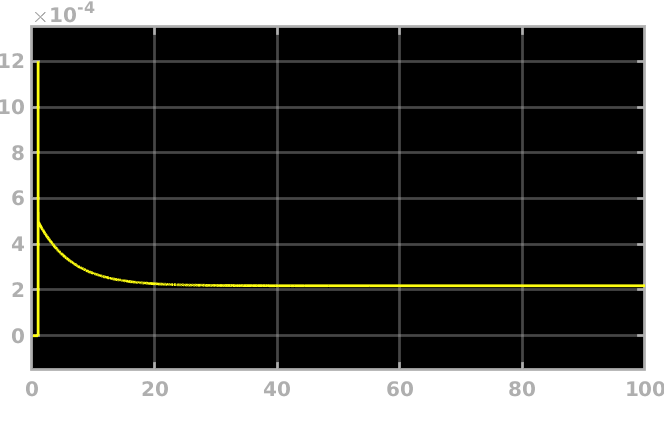
\includegraphics[width=\linewidth]{ukol3P0005DmaleIU}
    \caption{Průběh akčního zásahu u(t) ovládaným PD regulátorem s hodnotami P~=~0.005 a D~=~0.00007}
  \end{minipage}\hfill
  \begin{minipage}[b]{.45\textwidth}
    \centering
    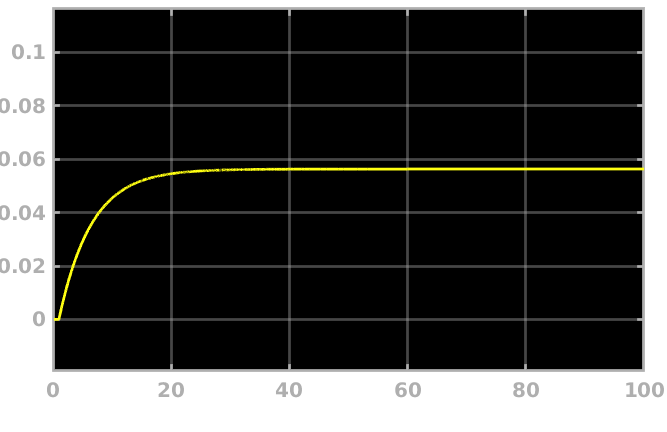
\includegraphics[width=\linewidth]{ukol3P0005DmaleIY}
    \caption{Průběh výšky hladiny systému y(t) regulovaným PD regulátorem s hodnotami P~=~0.005 a D~=~0.00007}
    \label{img:hladinaPD0005}
  \end{minipage}
	   		\end{figure}
	   		

	\indent Složku D jsem experimentálně nastavil na hodnotu 0.00007. Tato hodnota způsobuje impulz v počátku působení, kde se během časového okamžiku limitně blížícího se k 0s na vstupu objeví hodnota vstupu 1.2l/s, což přesahuje mnou zvolené maximum. Toto avšak zanedbám, protože se jedná o jev způsobený použitím prvku D.
	
	\subsection{Regulace pomocí složek PI}
	\paragraph{}
	
	Regulační složka I integruje hodnotu regulační odchylky a tuto hodnotu poté přičítá po vynásobením integrační konstanty k hodnotě akčního zásahu. Způsobí to, že se hodnota y(t) ustálí po delší době, ale ustálí se na hodnotě w(t). 
	
	
	\begin{figure}[H]
	   		 \begin{minipage}[b]{.45\textwidth}
    \centering
    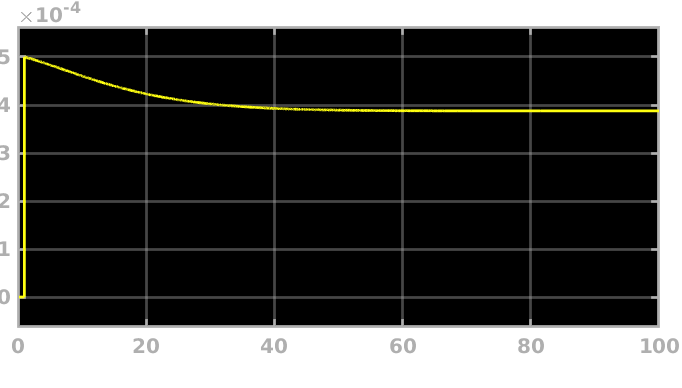
\includegraphics[width=\linewidth]{ukol3P0005I000048U}
    \caption{Průběh akčního zásahu u(t) ovládaným PI regulátorem s hodnotami P~=~0.005 a I~=~0.00048}
  \end{minipage}\hfill
  \begin{minipage}[b]{.45\textwidth}
    \centering
    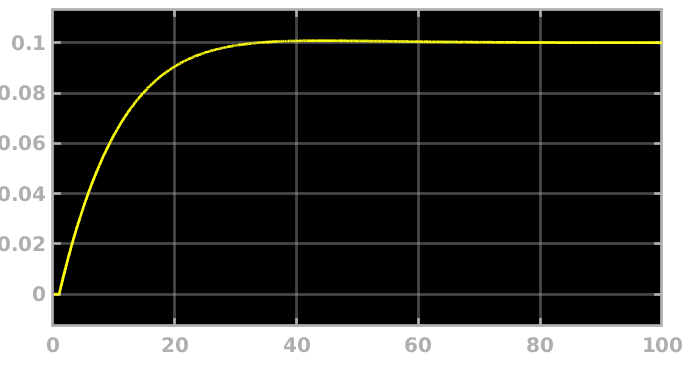
\includegraphics[width=\linewidth]{ukol3P0005I000048Y}
    \caption{Průběh výšky hladiny systému y(t) regulovaným PI regulátorem s hodnotami P~=~0.005 a I~=~0.00048}
    \label{img:hladinaPI0005}
  \end{minipage}
	   		\end{figure}
	   		
	   		
	   		Na grafu y(t) lze sledovat, že průbeh se oproti P, PI, PD regulaci ustálí na požadované hodnotě. Pokud integrační konstantu zvýšíme (z hodnoty 0.00048 na 0.00096), dojde k docela výraznému zákmitu regulované hodnoty a přesahu maximální hodnoty akčního zásahu. 
	   		

	\subsubsection{Regulace pomocí složek PID}
	\paragraph{}
	Pokud zkombinujeme všechny předešlé regulační složky, dostaneme experimentálně navolený PID regulátor. 
	
		   	
	\begin{figure}[H]
	   		 \begin{minipage}[b]{.45\textwidth}
    \centering
    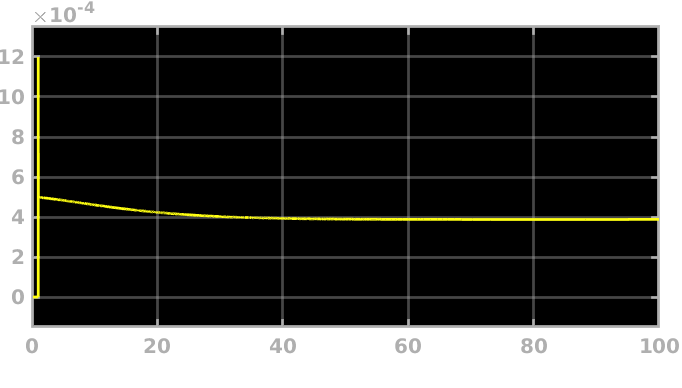
\includegraphics[width=\linewidth]{ukol3PIDu}
    \caption{Průběh akčního zásahu u(t) ovládaným PID regulátorem s hodnotami P~=~0.005 , I~=~0.00048 a D~=~0.00007}
  \end{minipage}\hfill
  \begin{minipage}[b]{.45\textwidth}
    \centering
    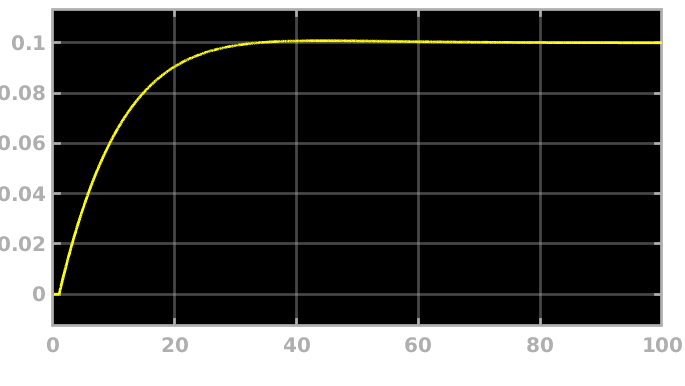
\includegraphics[width=\linewidth]{ukol3PIDy}
    \caption{Průběh výšky hladiny systému y(t) regulovaným PID regulátorem s hodnotami P~=~0.005, I~=~0.00048 a D~=~0.00007}
    \label{img:hladinaPID}
  \end{minipage}
	   		\end{figure}	
	   		
	   		Tento průběh vcelku rychle konverguje, což je dobrá vlastnost. Jediný nereálný jev je počáteční impulz sekce D. Tento jev je vysvětlen v sekci PD.
	   		
	   		
	   		% Please add the following required packages to your document preamble:
% \usepackage{graphicx}
\begin{table}[H]
\centering

\resizebox{0.25\textwidth}{!}{%
\begin{tabular}{|l|l|}
\hline
\textbf{Konstanta} & \textbf{Hodnota} \\ \hline
\textit{P}         & \textit{0.005}   \\ \hline
\textit{I}         & \textit{0.00048} \\ \hline
\textit{D}         & \textit{0.00007} \\ \hline
\end{tabular}%
}
\caption{Hodnoty konstant pro idealní PID}
\label{tab:pid_ideal}
\end{table}


\section{Úkol 4}
\subsection{Nastavení PID pomocí předešlých hodnot}
\paragraph{}
V tomto úkolu jsme měli jako první nastavit skutečný PID regulátor pomocí nastavených hodnot z úkolu č. 3. Po nastavení mi vyšly následující grafy:


\begin{figure}[H]
	   		 \begin{minipage}[b]{.45\textwidth}
    \centering
    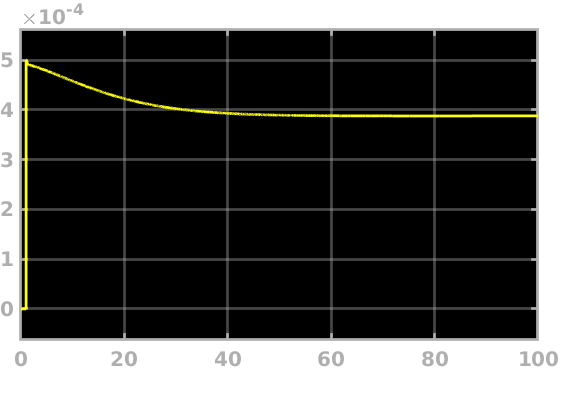
\includegraphics[width=\linewidth]{ukol4PIDu}
    \caption{Průběh akčního zásahu u(t) ovládaným reálným PID regulátorem s hodnotami P~=~0.005 , I~=~0.00048 a D~=~0.00007}
  \end{minipage}\hfill
  \begin{minipage}[b]{.45\textwidth}
    \centering
    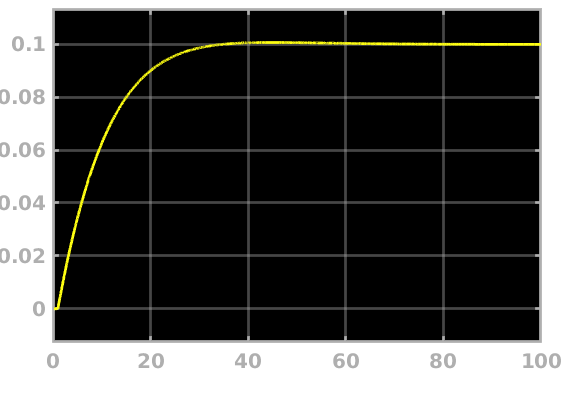
\includegraphics[width=\linewidth]{ukol4PIDy}
    \caption{Průběh výšky hladiny systému y(t) regulovaným reálným PID regulátorem s hodnotami P~=~0.005, I~=~0.00048 a D~=~0.00007}
    \label{img:hladinaPIDreal}
  \end{minipage}
	   		\end{figure}	
	   		
	   		
	\indent U prvního grafu lze sledovat, že oproti ideálnímu PID regulátoru zmizel původní impulz. Ve druhém grafu lze vidět, že jsou si průběhy skutečného a ideálního PID regulátoru identické.

\subsection{Nastavení PID podle experimentálně vyladěných hodnot}	
	
	\indent V další části jsme měli přenastavit PID tak, aby to regulovalo podle nás. Experimentálně jsem tedy nastavil následující hodnoty: 
	
	
	\begin{table}[H]
\centering
\resizebox{0.25\textwidth}{!}{%
\begin{tabular}{|l|l|}
\hline
\textbf{Konstanta} & \textbf{Hodnota} \\ \hline
\textit{P}         & \textit{0.35}   \\ \hline
\textit{I}         & \textit{0.01} \\ \hline
\textit{D}         & \textit{0.07} \\ \hline
\end{tabular}%
}
\caption{Odladěné hodnoty pro skutečný PID}
\label{tab:pid_ideal_lad}
\end{table}


	\indent Při těchto hodnotách systém konvergoval podstatně rychleji, protože jsme schopni propouštět maximální průtok bez obav, žebychom ho přestřelili, jak tomu bylo v Úkolu 3. Průběhy poté měli následující tvar:
	\begin{figure}[H]
	   		 \begin{minipage}[b]{.45\textwidth}
    \centering
    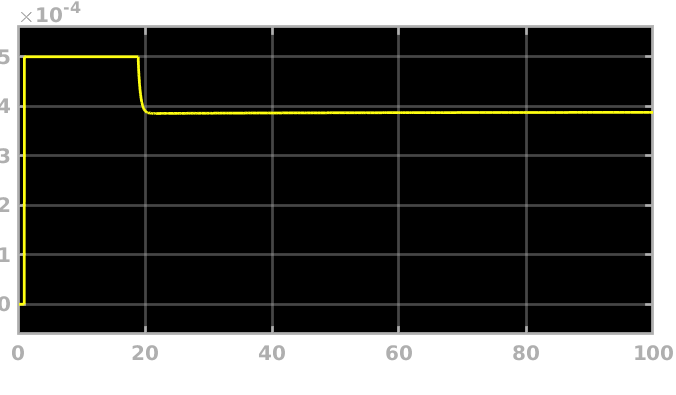
\includegraphics[width=\linewidth]{ukol4PIDuLAD}
    \caption{Průběh akčního zásahu u(t) ovládaným reálným odlaďěným PID regulátorem s hodnotami P~=~0.35 , I~=~0.01 a D~=~0.07}
  \end{minipage}\hfill
  \begin{minipage}[b]{.45\textwidth}
    \centering
    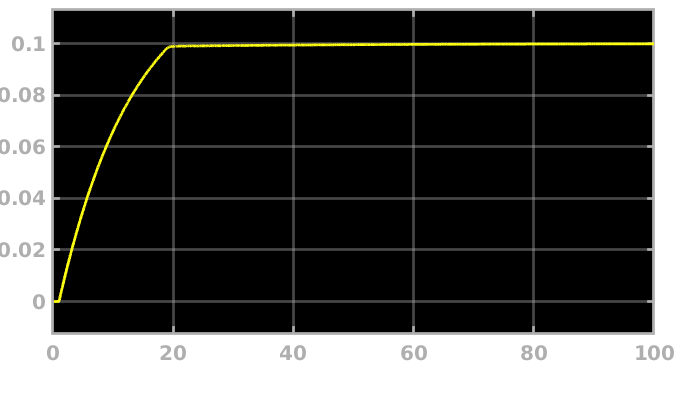
\includegraphics[width=\linewidth]{ukol4PIDyLAD}
    \caption{Průběh výšky hladiny systému y(t) regulovaným reálným odlaďěným PID regulátorem s hodnotami P~=~0.35 , I~=~0.01 a D~=~0.07}
    \label{img:hladinaPIDrealLAD}
  \end{minipage}
	   		\end{figure}	
	
	\begin{figure}[H]
 	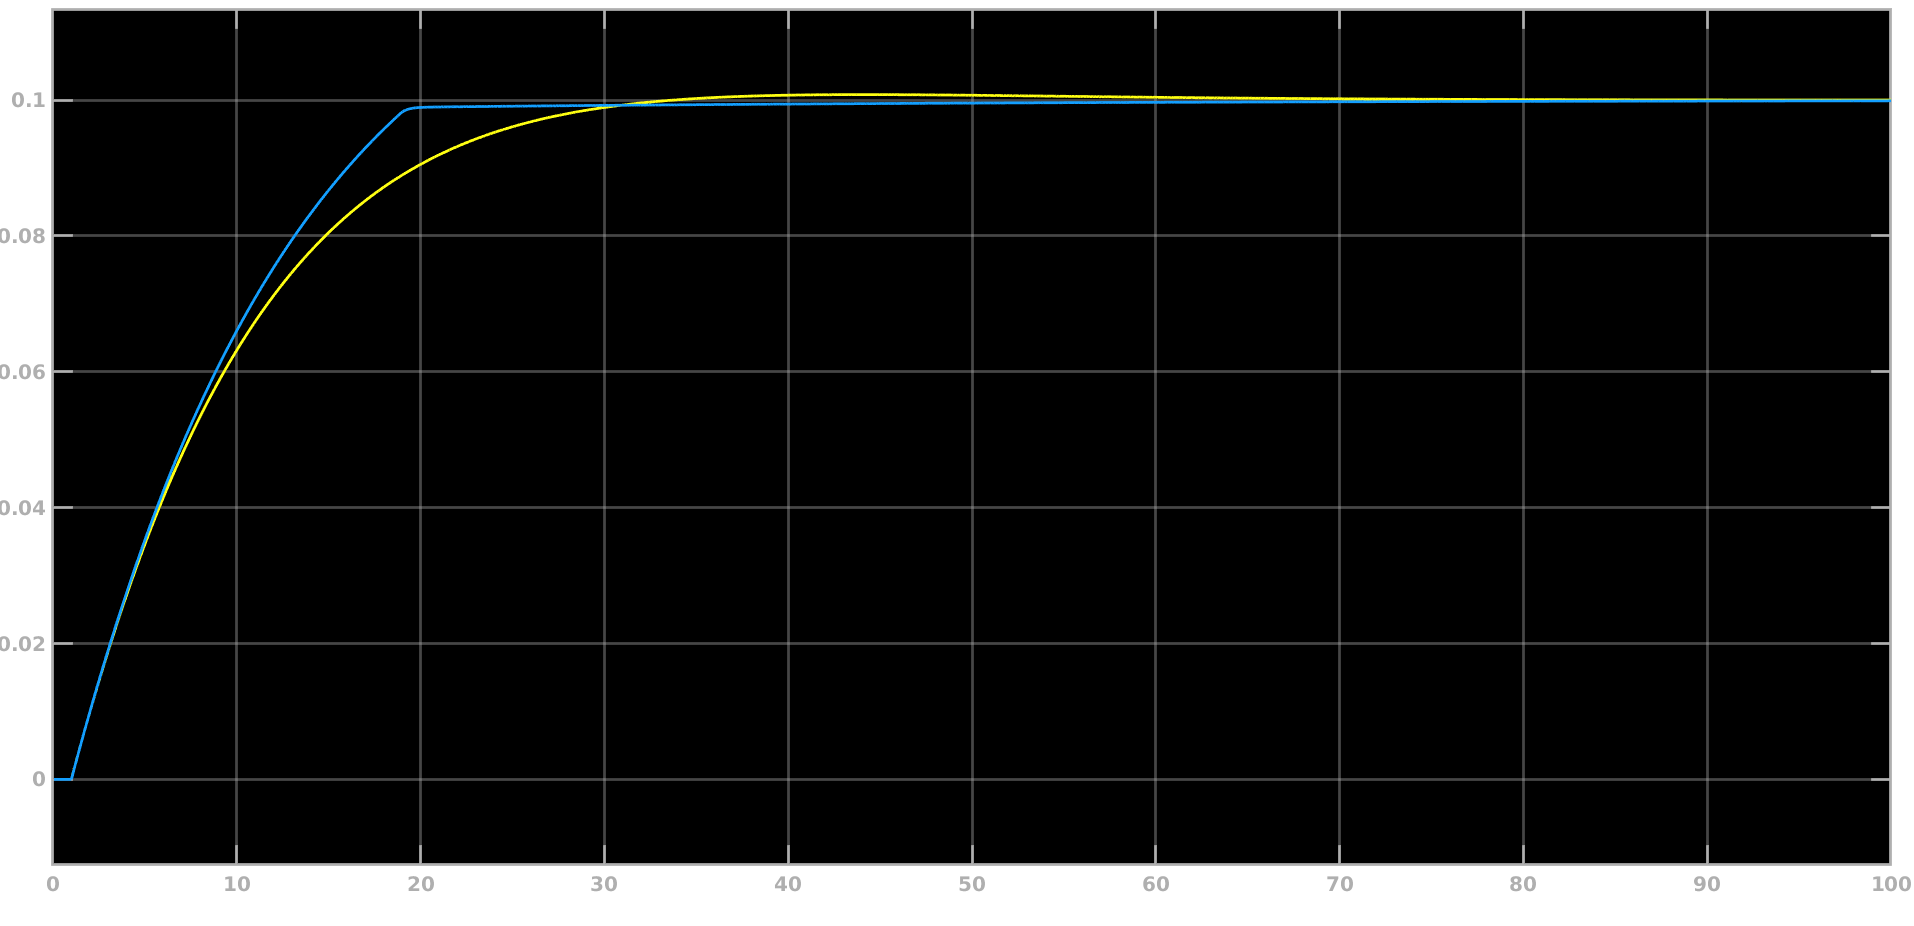
\includegraphics[width=\textwidth]{ukol4comp}
 	\caption{Porovnání regulace laděné na ideálním PID regulátoru (žlutá) a skutečném PID regulátoru (modrá)}
 	\end{figure}
   			

	\section{Úkol 5}
	\subsection{Porovnání vlivu PID na nelineární a LTI systém}
	\paragraph{}	
	V tomto úkolu jsme měli použít regulátor z předchozí úlohy na nelineární systém, který jsme nahradili lineárním v úloze 1.  Simulací nelineárního systému v porovnáním s náhradním lineárním systémem jsem zjistil, že má delší dobu ustálení při nárůstu, ale nižší dobu ustálení při poklesu. Toto jsem nasimuloval tak, že jsem požadovanou výšku w(t) v čase t=0 nastavil na hodnotu 0.1m, a v čase t=50s jsem ji přenastavil na hodnotu 0.05m. Tímto jsme dostali následující průběhy akční veličiny u(t) a regulované veličiny y(t). Pokud se podíváme na průběhy akčních veličin u(t) a (Obrázek~\ref{img:akcnivel_realita}), můžeme sledovat, že u průběhu akčního zásahu u nelineárního systémů se nádrž naplňuje delší dobu, a je zapotřebí pro udržení hladiny na požadované hodnotě je zapotřebí vyšší průtok. Naopak pokud hladinu chceme snížit, bude zapotřebí menší časový okamžik. Lze zde taky sledovat to, že je zapotřebí daleko vyšší průtok pro udržení nižší hladiny. Toto je pravděpodobně způsobeno zanedbáním druhé odmocniny u LTI modelu.
	
	
		\begin{figure}[H]
		\centering
 	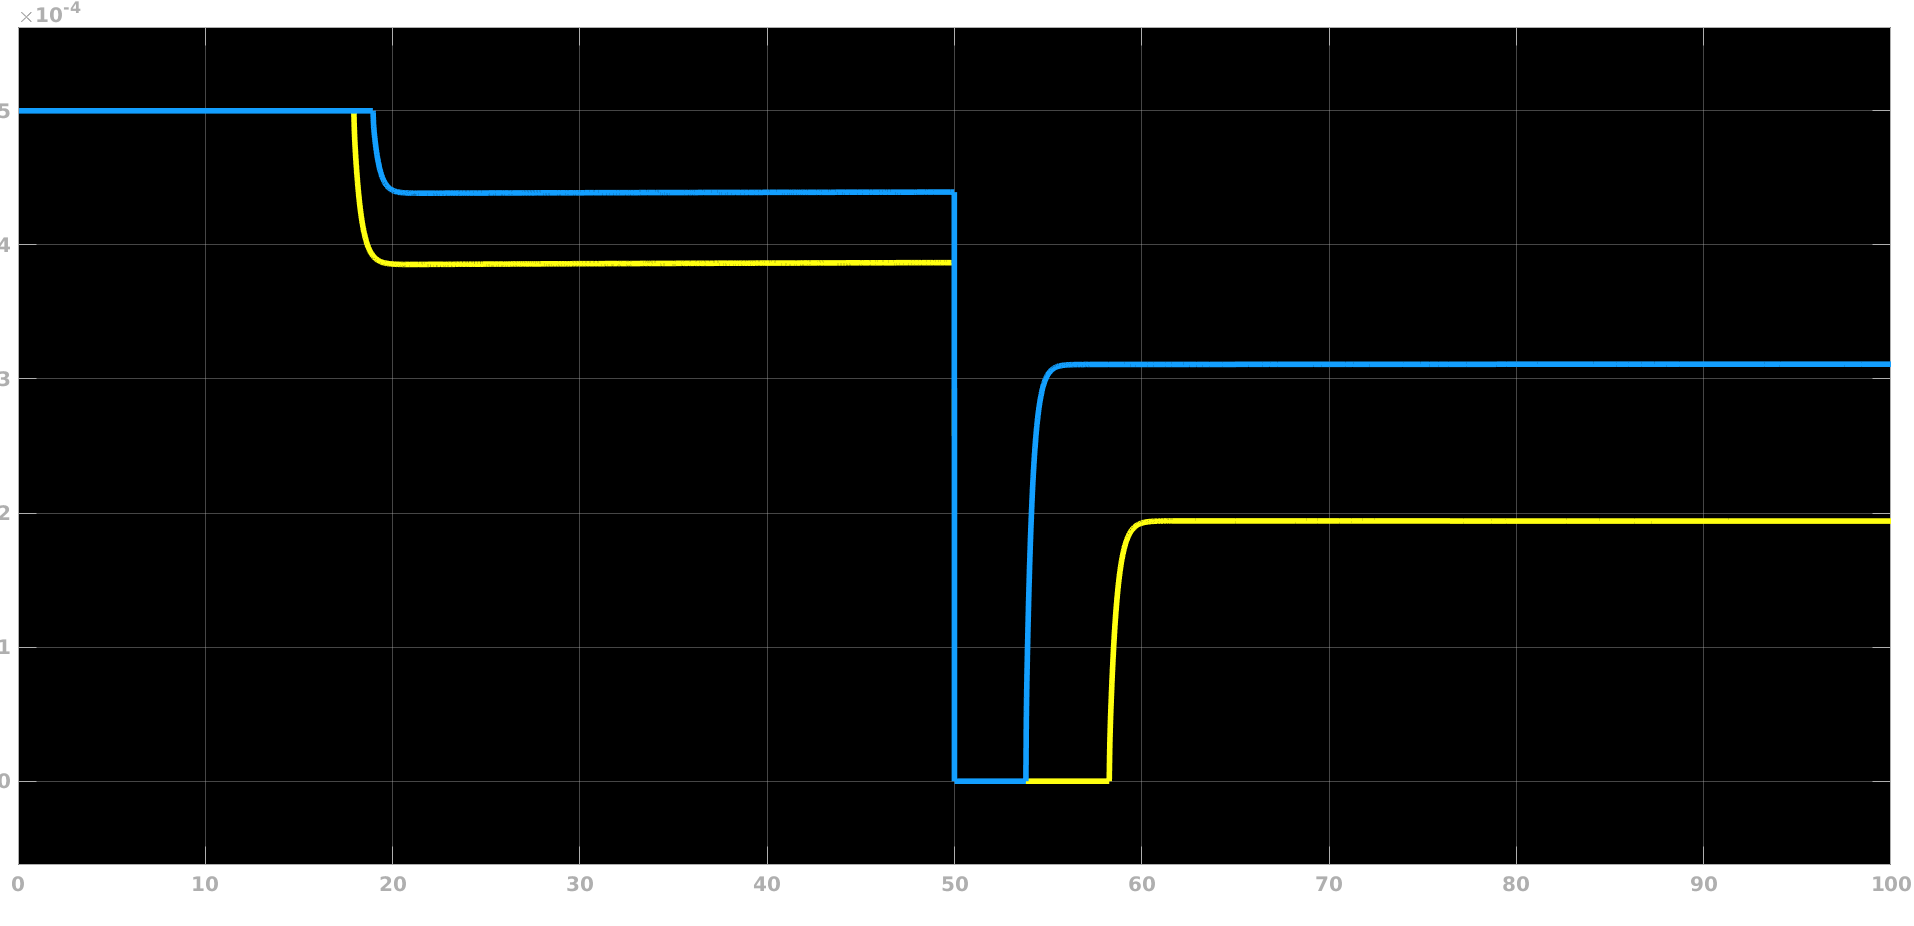
\includegraphics[width=0.8\textwidth]{ukol5uComp}
 	\caption{Průběhy akčních zásahů nelineárního a LTI systému regulovaných PID regulací s upravou w(t) v čase 50s na polovinu požadované hodnoty}
 	\label{img:akcnivel_realita}
 	\end{figure}
 	\begin{figure}[H]
 	\centering
 	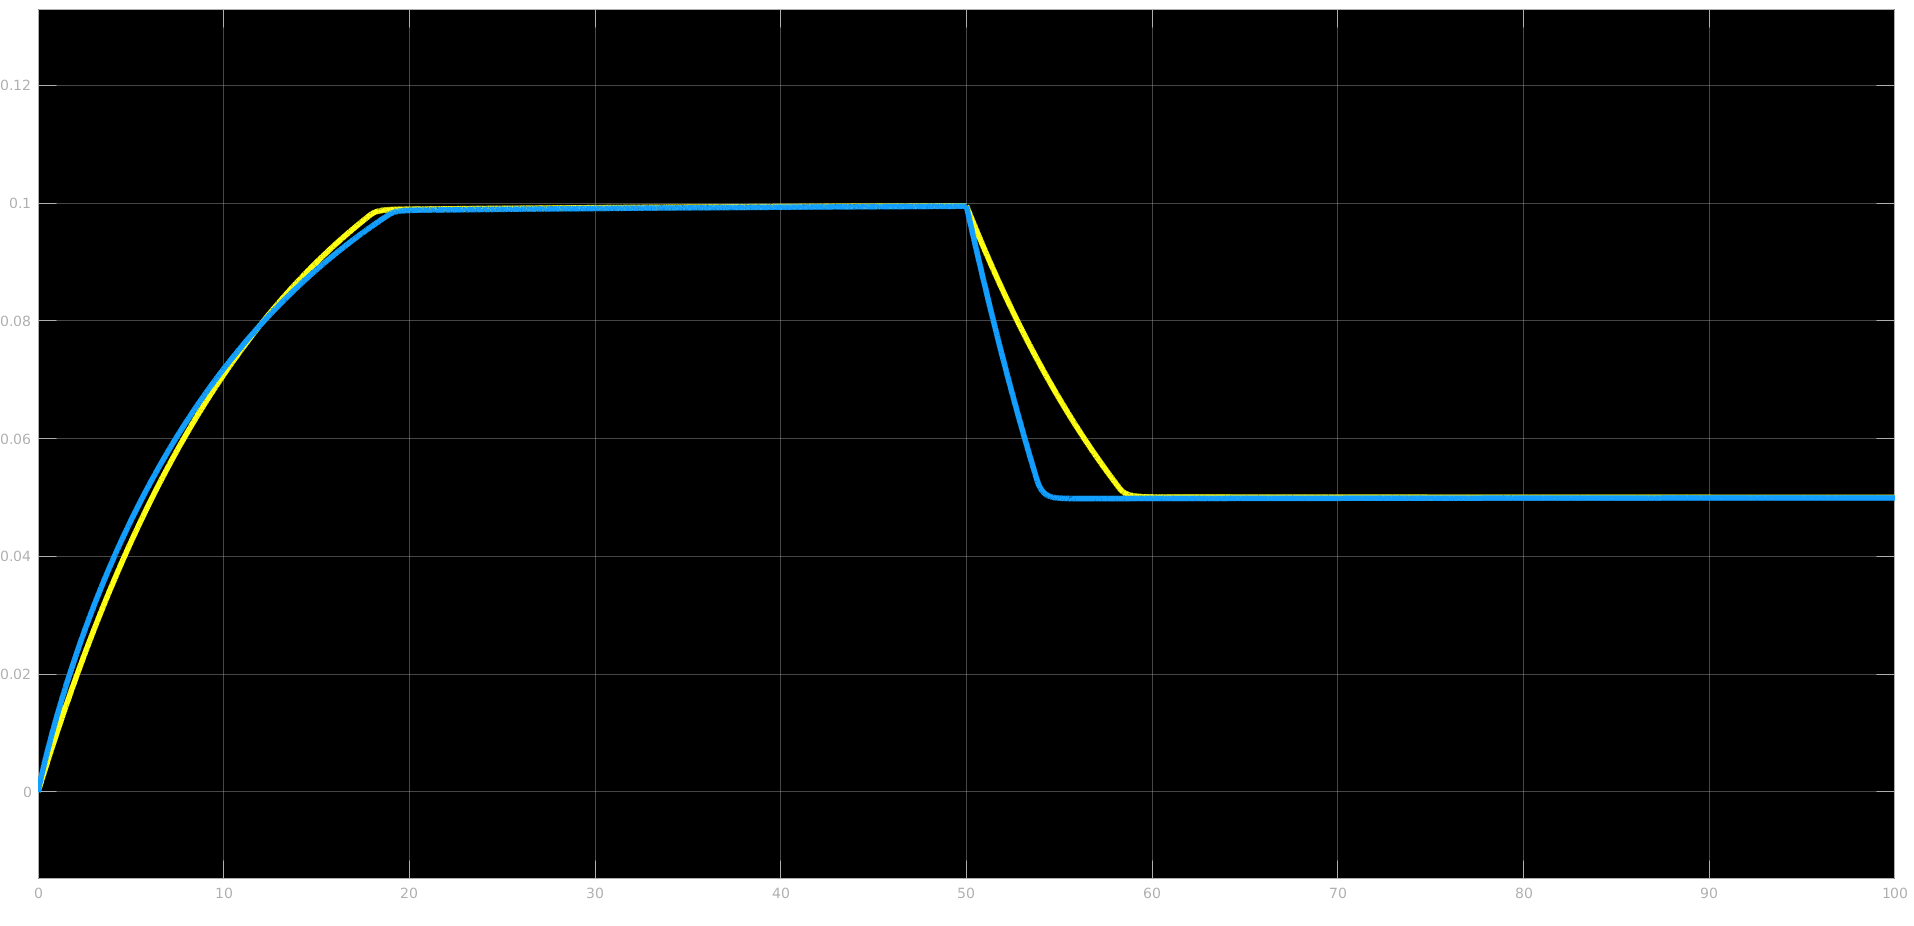
\includegraphics[width=0.8\textwidth]{ukol5yComp}
 	\caption{Průběhy regulovaných veličin nelineárního a LTI systému regulovaných PID regulací s upravou w(t) v čase 50s na polovinu požadované hodnoty}
 	\end{figure}
 	
 	
	
	\section{Úkol 6}
	
	
	\subsection{Popis bloku Relay s hysterezí}
	\paragraph{}
	V této sekci budeme realizovat regulaci tohoto systému pomocí ON/OFF regulace. Pro realizaci této regulace budeme využívat	 blok Relay s hysterezi. Zkoumáním dokumentace MATLab Simulinku jsem zjistil, že Relay blok má 4 parametry. Tyto parametry mají následující charaktery dle mnou vytvořené tabulky.
	
	% Please add the following required packages to your document preamble:
% \usepackage{graphicx}
\begin{table}[H]
\centering
\resizebox{\columnwidth}{!}{%
\begin{tabular}{|l|l|l|}
\hline
\textbf{Název pole v Simulinku} & \textbf{Veličina} & \textbf{Popis}                        \\ \hline
Switch on point  & e(t) & \begin{tabular}[c]{@{}l@{}}Minimální velikost regulační odchylky, při které\\ dochází k sepnutí relay.\end{tabular} \\ \hline
Switch off point & e(t) & \begin{tabular}[c]{@{}l@{}}Velikost regulační odchylky, při které dochází k\\ vypnutí relay\end{tabular}            \\ \hline
Output when on                  & u(t)              & Velikost průtoku při sepnutém relay   \\ \hline
Output when off                 & u(t)              & Velikost průtoku při rozepnutém relay \\ \hline
\end{tabular}%
}
\caption{Legenda k Relay s Hysterezí}
\label{tab:simulink}
\end{table}
	
	\subsection{Realizace ON/OFF regulace pomocí bloku Relay s hysterezí}
	\paragraph{}
	Nejprve je nutné si určit, jak přesně chceme mít naregulovanou výsku hladiny. Já jsem si určil, že hladinu chci udržovat v rozsahu $\pm$2.5mm (resp. 0.0025m). Průtok, kterým budeme regulovat je 0.5l/s, což musím také nastavit v nastavení bloku relay s hysterezí. Pro tuto funkčnost nastavíme hodnoty bloku relay s hysterezí dle následující tabulky. Pod tabulkou je také zobrazen průběh u(t) a y(t).
	
	% Please add the following required packages to your document preamble:
% \usepackage{graphicx}
\begin{table}[H]
\centering
\resizebox{0.6\textwidth}{!}{%
\begin{tabular}{|l|l|l|}
\hline
\textbf{Název pole v Simulinku} & \textbf{Veličina} & \textbf{Hodnota} \\ \hline
Switch on point                 & e(t)              & 0.0025           \\ \hline
Switch off point                & e(t)              & -0.0025          \\ \hline
Output when on                  & u(t)              & 0.0005           \\ \hline
Output when off                 & u(t)              & 0                \\ \hline
\end{tabular}%
}
\caption{Nastavení bloku Relay s hysterezí}
\label{tab:nastaveni_relay}
\end{table}

\begin{figure}[H]
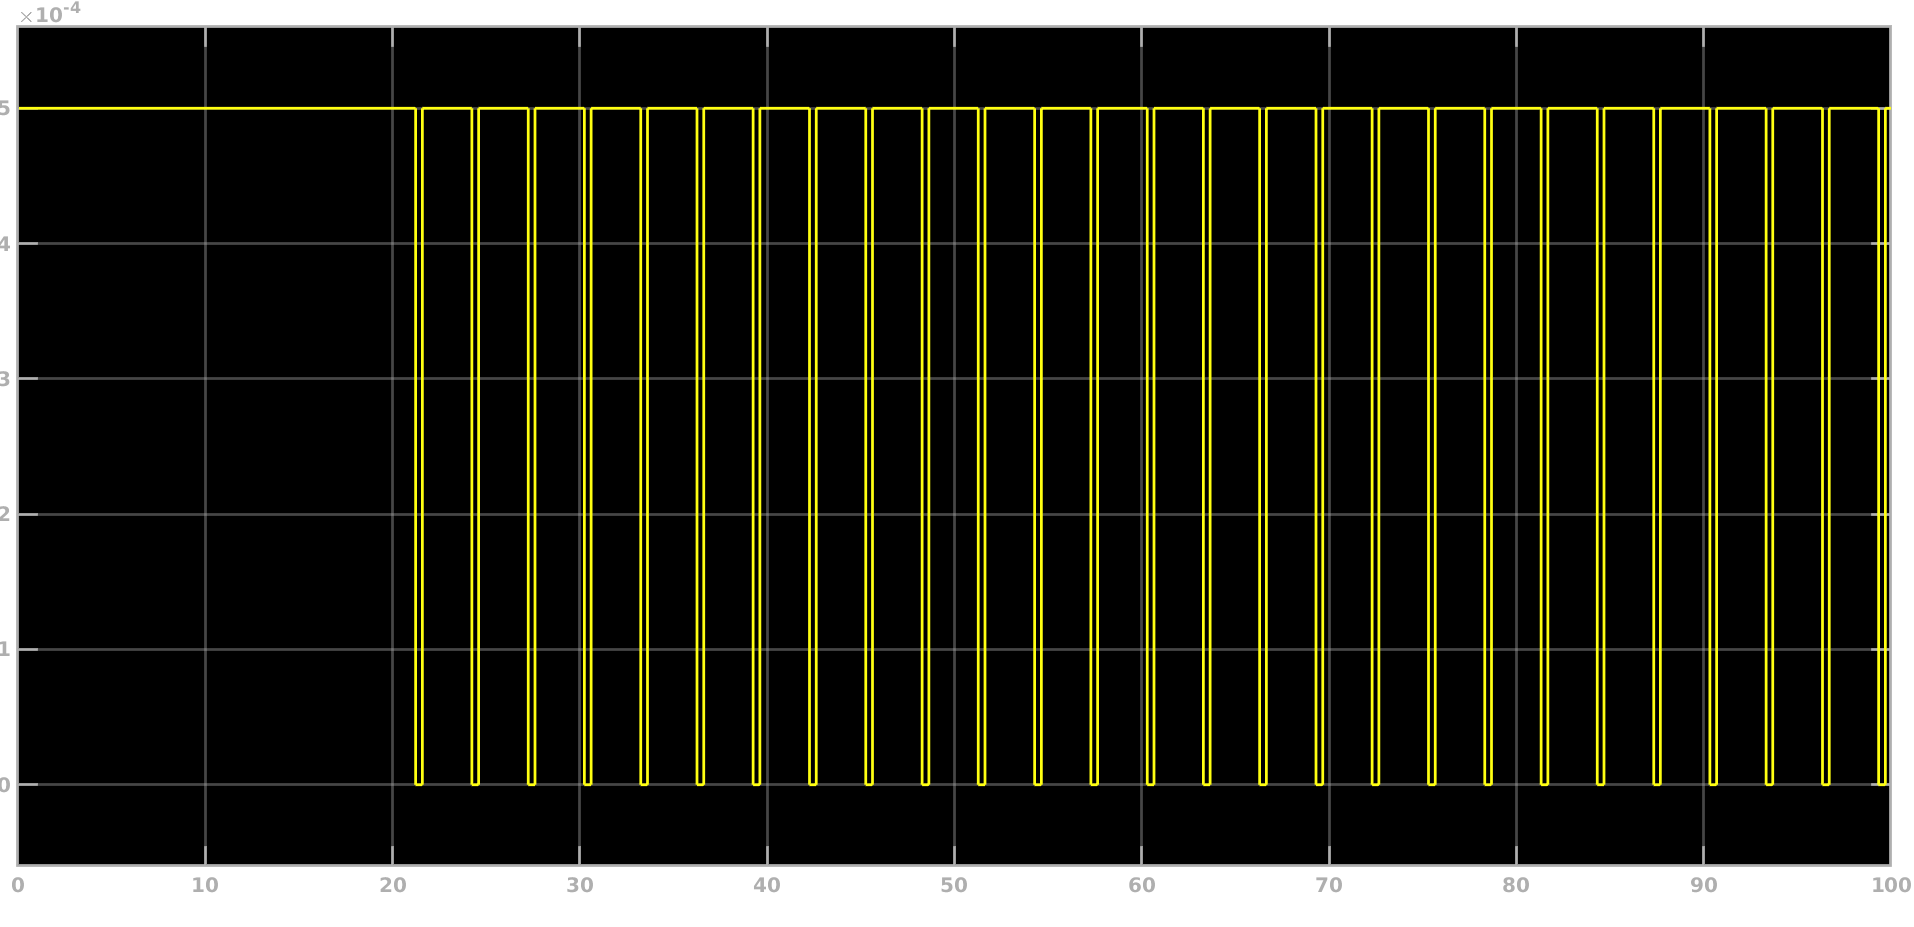
\includegraphics[width=\textwidth]{ukol6u}
\centering
\caption{Průběhy akčních zásahů u(t) nelineárního systému regulovaného pomocí PID regulátoru (žlutá) a ON/OFF regulátoru (modrá)}
\label{img:ut_onoff}
\end{figure}


\begin{figure}[H]
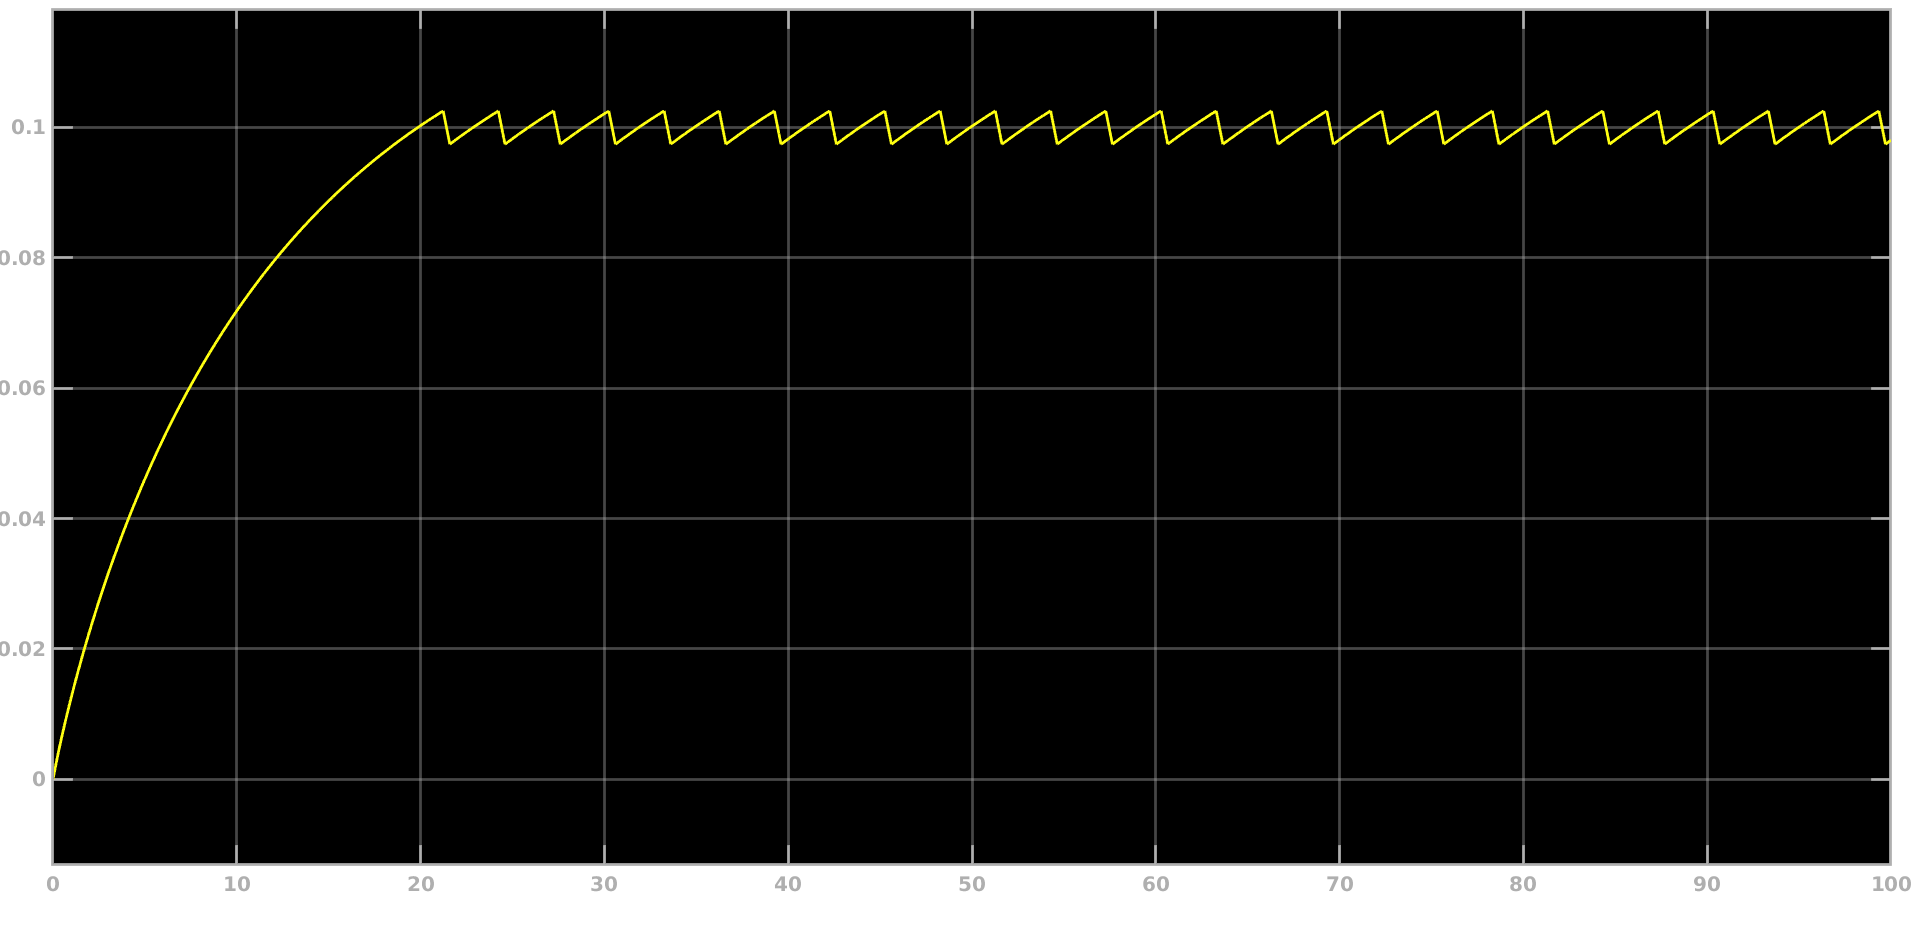
\includegraphics[width=\textwidth]{ukol6y}
\centering
\caption{Průběhy regulované veličiny y(t) nelineárního systému regulovaného pomocí PID regulátoru (žlutá) a ON/OFF regulátoru (modrá)}
\label{img:yt_onoff}
\end{figure}


\indent Na těchto grafech můžeme vidět, že tento způsob regulace reguluje v rozsahu kolem požadované hodnoty tak, jak jsme ho nastavili. Výstupní signál osciluje kolem požadované hodnoty. V tomto případě dochází avšak k přesahu, neboli k záporné hodnotě odchylky e(t). Toto nemusí být vyloženě špatně, ale může docházet kvůli tomuto k nekonečnému přetékání nádrže. Tomute jo však možno jednoduchými limitacemi rozsahu vstupní veličiny (V tomto případě např. omezit rozsah w(t) na <0.0025,~(max. výska nádrže)-0.0025>).

\subsection{Porovnání ON/OFF regulátoru s PID regulátorem}
\paragraph{}
	\indent V této části si porovnáme 2 již vytvořené regulace proti sobě. Na následujících grafech je zobrazen průběh dvou regulátorů (PID a ON/OFF) působící na dva shodné nelineární systémy. Vstupní signál požadované hodnoty budu používat stejný jako v úkolu č. 5, tzn. signál s prvotní požadovanou hodnotou 0.1m, který se v časovém okamžiku t=50s změní na hodnotu 0.05m.
	

\begin{figure}[H]
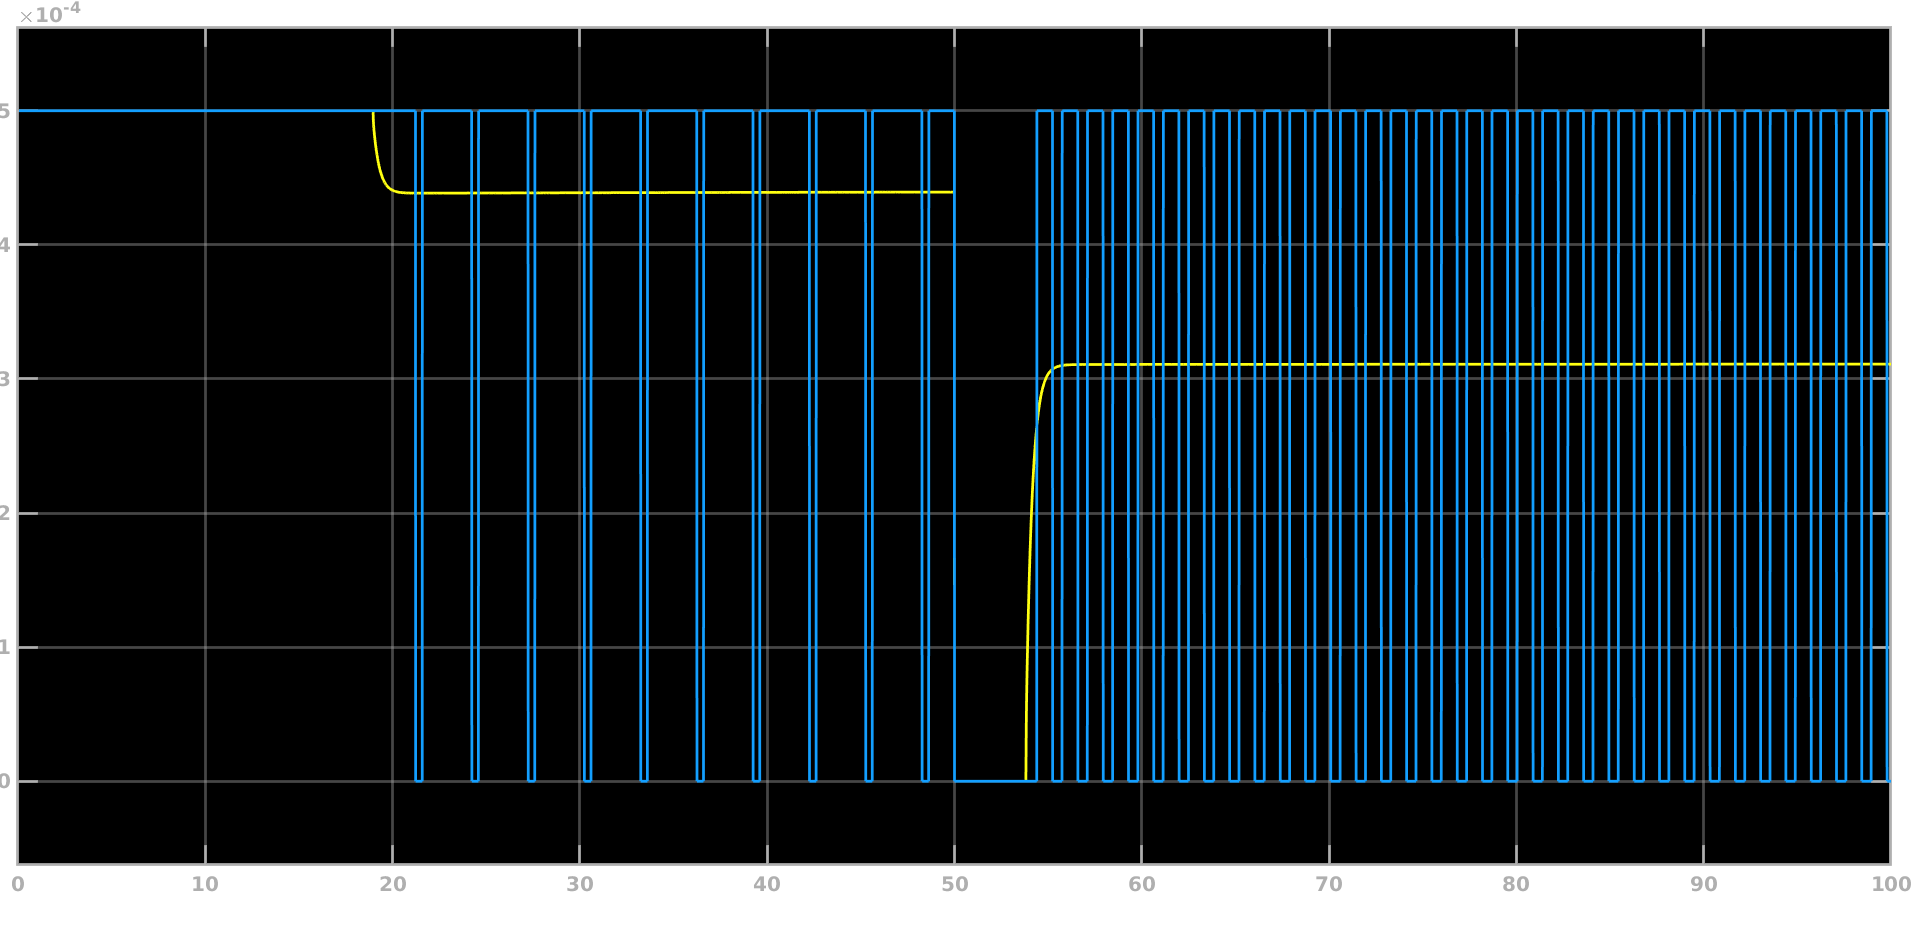
\includegraphics[width=\textwidth]{ukol6uComp}
\centering
\caption{Průběhy regulované veličiny y(t) nelineárního systému regulovaného pomocí PID regulátoru (žlutá) a ON/OFF regulátoru (modrá)}
\label{img:ut_onoffVSpid}
\end{figure}

\begin{figure}[H]
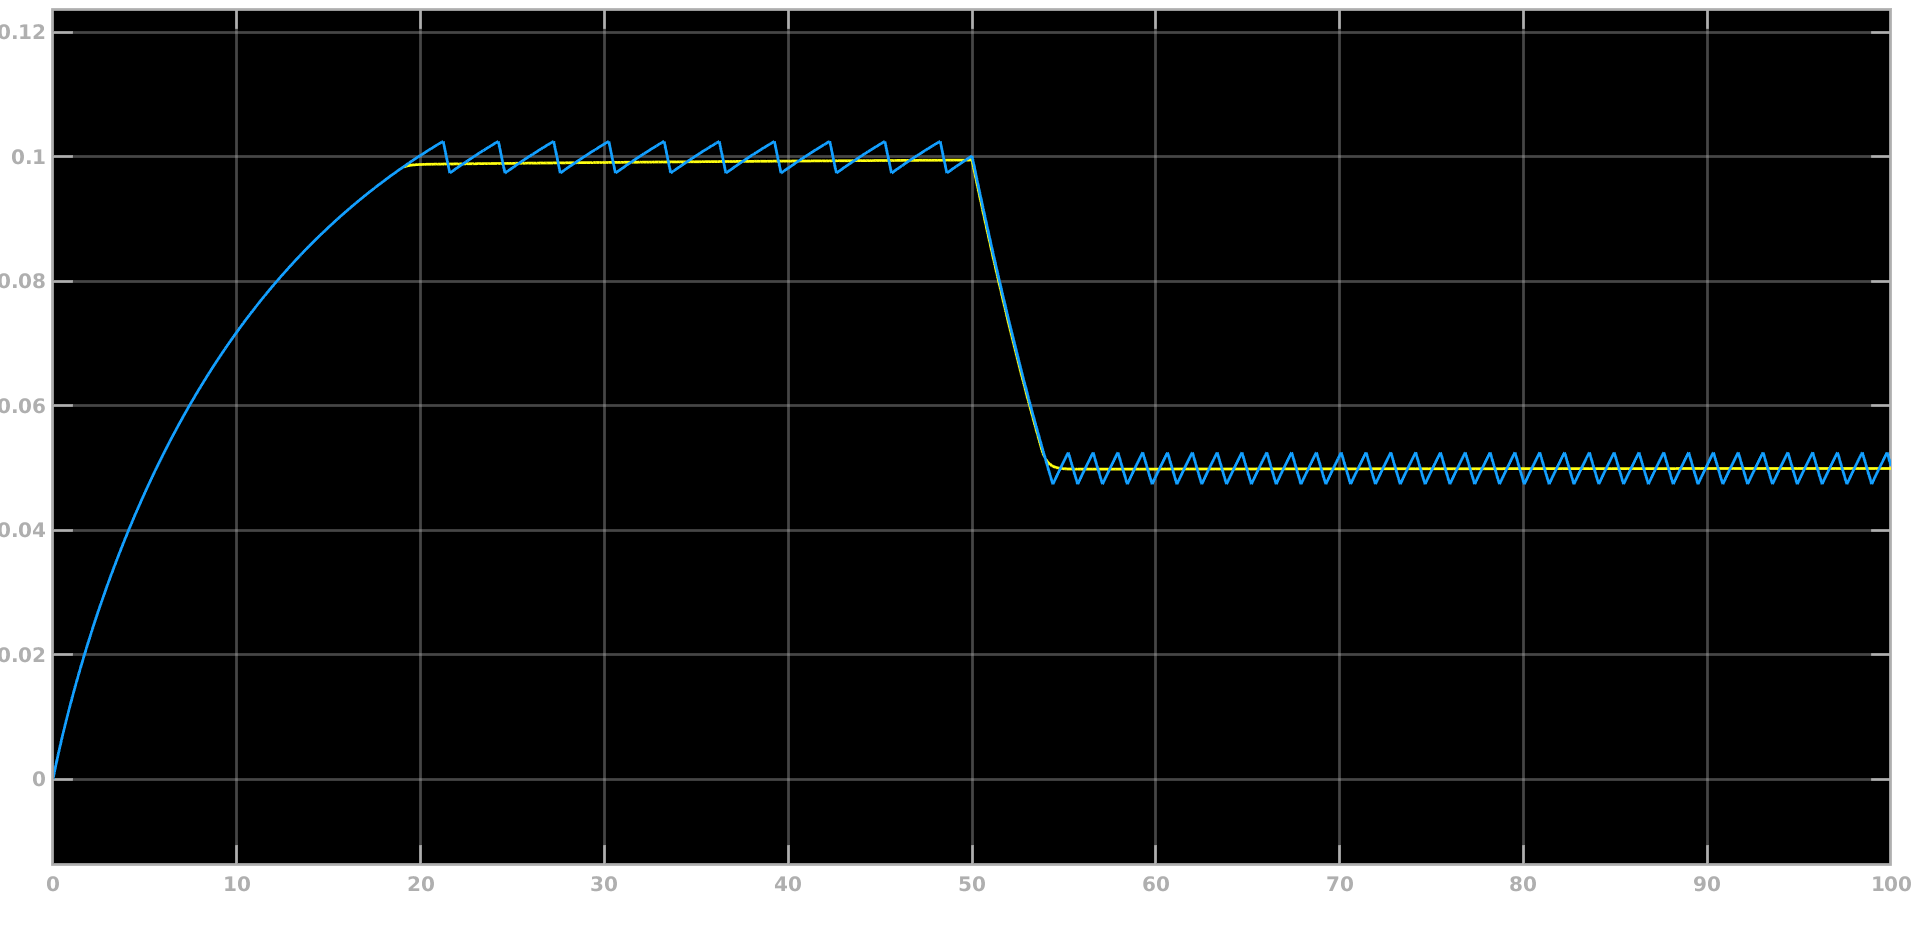
\includegraphics[width=\textwidth]{ukol6yComp}
\centering
\caption{Průběhy regulované veličiny y(t) nelineárního systému regulovaného pomocí PID regulátoru (žlutá) a ON/OFF regulátoru (modrá)}
\label{img:yt_onoffVSpid}
\end{figure}


\indent Na těchto grafech jde vidět, že ON/OFF regulátor dosáhne požadované hodnoty ve stejnou dobu jako regulátor PID.

\section{Závěr}
\paragraph{}
Simulacemi provedenými v tomto projektu jsme si objasnili jak funguje PID regulace a jak se experimentálně nastavují její parametry. Pro samotné nastavování parametrů jsme první nahradili nelineární systém systémem LTI. Parametry tohoto systému je možno nálézt v tabulce (tab.~\ref{tab:regtable}).
\indent Poté jsme nastavovali složku P, a pokud bychom regulovali pouze pomocí této složky, nikdy bychom nedosáhli očekávané hodnoty. Dále jsme nastavovali složku D v zapojení PD. Obvod se choval téměř stejně, jako u samotné složky P kvůli charakteru derivační složky. Závěrem jsme nastavovali složku I, která nám zajistila, že se v nějakém časovém okamžiku dostaneme do požadované hodnoty. Závěrem experimentálního nastavování jsme tyto nastavené hodnoty zkombinovaly do ideálního PID rehulátoru, který zkombinoval všechny vlastnosti předešlých systémů. Nastavené hodnoty jsou možny vidět v tabulce (tab~\ref{tab:pid_ideal}).\\
\indent Tyto hodnoty jsme následně nastavili do reálného PID regulátoru. Ten měl následně totožný průběh jako měl průběh ideální. Poté, co jsem tyto konstanty změnil na experimentálně odladěnější hodnoty (tab~\ref{tab:pid_ideal_lad}) jsem tyto dva regulátory porovnal, a zjistil, že při laděném reálném PID regulátoru dosáhl obvod požadované hodnoty zhruba o 10s dříve. \\
\indent Následně jsem tento regulátor zkusil aplikovat na nelineární systém. Tento systém reguloval s různými rychlostmi konvergence pro stoupání nebo klesání, a potřeboval vyšší průtok pro udržení stálé hladiny. Toto bylo pravděpodobně způsobeno nelinearitou druhé odmocniny.\\
\indent Závěrem jsem si zkusil nastavení ON/OFF regulátoru pro stejný nelineární systém. Nastavoval jsem to tak, aby se výsledná hodnota pohybovala $\pm$2.5mm kolem požadované hodnoty. Nastavení ON/OFF regulace je uvedeno v tabulce (tab.~\ref{tab:nastaveni_relay}). Toto způsobilo po dosažení požadované hodnoty pilovitý průběh okolo požadované hodnoty. Při porovnání tohoto způsobu regulace oproti PID jsem zhodnotil, že ON/OFF regulace je horší na stav ovládání průtuku, jelikož ho velmi často musím celý otevřít a zavřít. Tímto namáháním by se mohl rychle opotřebit, což u PID regulace zas takový problém nebude. Veliký problém PID regulace je avšak jeho cena, tudíž si dovedu představit použití ON/OFF regulace, realizované pomocí levného mikročipu a relátka, na místa, kde rozhoduje cena.


    \renewcommand{\sectionmark}[1]{\markright{#1}}
    \cleardoublepage
    \appendix
    \pretocmd{\chapter}{\pagenumbering{arabic}
	                          \renewcommand*{\thepage}{\thechapter.\arabic{page}}
                           }{}{} 
    \include{appendix1}
\end{document}